\documentclass{isnotes}
\usepackage[spanish]{babel}

\classname{IS-210}
\professor{Servio Paguada}
\title{Título de la nota}

\begin{document}
\maketitle

\section{Paquetes requeridos por la clase}
\begin{itemize}
	\item xcolor
	\item graphicx
	\item minted
\end{itemize}

Además de los paquetes de la lista anterior, esta clase las fuentes \textbf{Chivo} y \textbf{Roboto}, que estan incluidas en la instalación de TexLive

\section{Secciones}
Contenido de la sección

\section{Subsecciones}

El siguiente ejemplo es de una subsección

\subsection{Esta es una subsección con la opciones por defecto}

Texto de la subsección

\section{Código}
Para escribir código se require tener instalado el paquete minted. Por ahora no se puede establecer la tabulación del código a través de las opciones de la clase, pero es posible cambiarla en el entorno de cada languaje, mediante las opciones del paquete minted, e.g. \textbf{tabsize}. Ver entorno \textbf{cppcode} en isnotes.cls

\begin{listing}[ht!]
\begin{javacode}
public class Prueba {
	public static void main(String[] args) {
		int valor = 1;
	}
}
\end{javacode}
\end{listing}

\section{Imagenes}
Las imágenes deberán ser incluidas con el entorno \textbf{Figure}.

\begin{figure}[ht!]
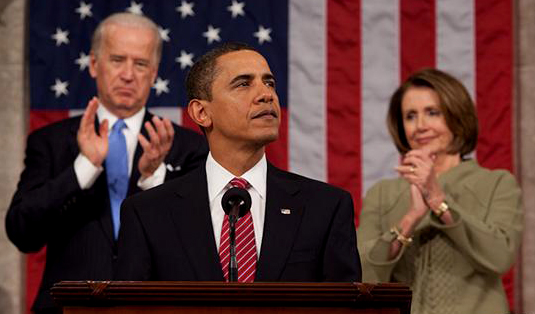
\includegraphics[width=\textwidth]{images/obama.png}
\end{figure}





\end{document}